\chapter{Interaction of multiple selected loci.}

Consider two biallelic loci segregating for $A/a$ and $B/b$. There are four haplotypes $AB$, $Ab$, $aB$, $ab$, which for simplicity we label 1-4. The frequency of our four haplotypes are $x_1$, $x_2$, $x_3$, and $x_4$. Each individual has a genotype consisting of two haplotypes, we label $w_{ij}$ the fitness of an individual with the genotype made up of haplotype $i$ and $j$ (we assume that $w_{ij}=w_{ji}$, i.e. there are no parent of origin effects). Assuming that these fitnesses reflect differences due to viability selection, and that individuals mate at random, we can write the following table of our genotype proportions after selection:\\
\begin{center}
\begin{tabular}{c|cccc}
         & $AB$			& $Ab$				& $aB$				& $ab$\\
\hline
$AB$ & $w_{11} x_1^2$ 	& $w_{12} 2 x_1 x_2$  	& $w_{13} 2 x_1 x_3$ 	& $w_{14} 2 x_1 x_4$ \\
$Ab$ & $\bullet$ 	  	& $w_{22} x_2^2$ 	  	& $w_{23} 2 x_2 x_3$  	& $w_{24} 2 x_2 x_4$ \\  
$aB$ & $\bullet$ 		& $\bullet$ 			& $w_{33} x_3^2$ 	  	& $w_{34} 2 x_3 x_4$ \\  
$ab$ & $\bullet$ 		& $\bullet$			& $\bullet$ 			&  $w_{44} x_4^2$ \\
\end{tabular}
\end{center}
This follows from assume that our haplotypes are brought together at random (HWE) then discounted by their fitnesses. Our mean fitness $\bar{w}$ is the sum of all the entries in the table, which normalized the complete table to sum to one. The frequency of $AB$ haplotype ($1$) in the next generation of gametes is
\begin{equation}
x_1' = \frac{\big( w_{11} x_1^2 +	 \half w_{12} 2 x_1 x_2  + \half w_{13} 2x_1 x_3  +	 \half (1-r) w_{14} 2 x_1 x_4 + \half r w_{23} 2 x_2 x_3   \big)}{ \bar{w} } \label{eqn:hapfreq}
\end{equation}
Here each of the HWE genotype frequencies (e.g. $2x_1x_2$) is weighted by their fitness relative to the mean fitness ($w_{ij}/\bar{w}$), and by their probability of transmitting the AB haplotype to the next generation, for example $AB/Ab$ individuals (1/2) transmit the $AB$ haplotype only half the time. The final two terms include the recombination fraction ($r$). The first term involving recombination refers to the $AB/ab$ genotype (1/4), who with probability $(1-r)/2$ transmit a non-recombinant $AB$ haplotype to the gamete. Similarly the second term refers to a  $Ab/aB$ genotype, a proportion $r/2$ of their gametes carry the recombinant $AB$ haplotype. 

In the single locus case we defined the marginal fitness of an allele, here it will help us to define the mariginal fitness of the $i^{th}$ haplotype
\begin{equation}
\bar{w}_i = \sum_{j=1}^4 w_{ij} x_j
\end{equation}
this is the fitness of the $i^{th}$ haplotype averaged over all of the genotypes it could occur in, weighted by their probability under random mating. Using this notation, and with some rearrangement of equation \eqref{eqn:hapfreq}, we obtain
\begin{equation}
x_1' = \frac{x_1\bar{w}_1 - w_{14} r D}{\bar{w}}
\end{equation}
here we have assumed that $w_{23}=w_{14}$, i.e. that the fitness of $AB/ab$ individuals is the same as $Ab/aB$ individuals (i.e. that fitness depends only on the alleles carried by an individual, and not on which chromosome they are carried, this assumption is sometimes called no {\it cis}-epistasis). 

We can then write the change in the frequency of our $1$ haplotype as 
\begin{equation}
\Delta x_1= \frac{x_1(\bar{w}_1-\bar{w}) -r w_{14} D}{\bar{w}}
\end{equation}
Generalizing from this we write the change in our set of four haplotypes as
\begin{equation}
\Delta x_i= \frac{x_1(\bar{w}_i-\bar{w}) \pm r w_{14} D}{\bar{w}}
\end{equation}
where the coupling haplotypes 1 and 4 use $+D$ and repulsion haplotypes 2 and 3 use $-D$. Note that the sum of these four $\Delta x_i$ is zero, as our allele frequencies sum to one.

So the change in the frequency of a haplotype (eg AB, haplotype 1) is determined by the interplay of two factors. First the extent to which  the marginal fitness of our haplotype is higher (or lower) than the mean fitness of the population (the magnitude and sign of $(\bar{w}_1-\bar{w})/\bar{w}$). Second whether there is a deficit or any excess of our haplotype compared to linkage equilibrium (the magnitude and sign of $D$) modified by the strength of recombination. 

\subsection{Types of interaction between selection and recombination}

\paragraph{Interference.}



HIV uses its reverse transcriptase (RT) gene to write itself from an RNA virus into its host's DNA, allowing it to hijack the hosts regulatory machinary, a critical part of its life cycle. 
Efavirenz is an anti-HIV drug, which inhibts HIV's RT protein. Sadly mutations are common in the RT HIV gene, and in the presence of the drug have a profound fitness advantage alllowing them to spread. 

\begin{figure}
\begin{center}
  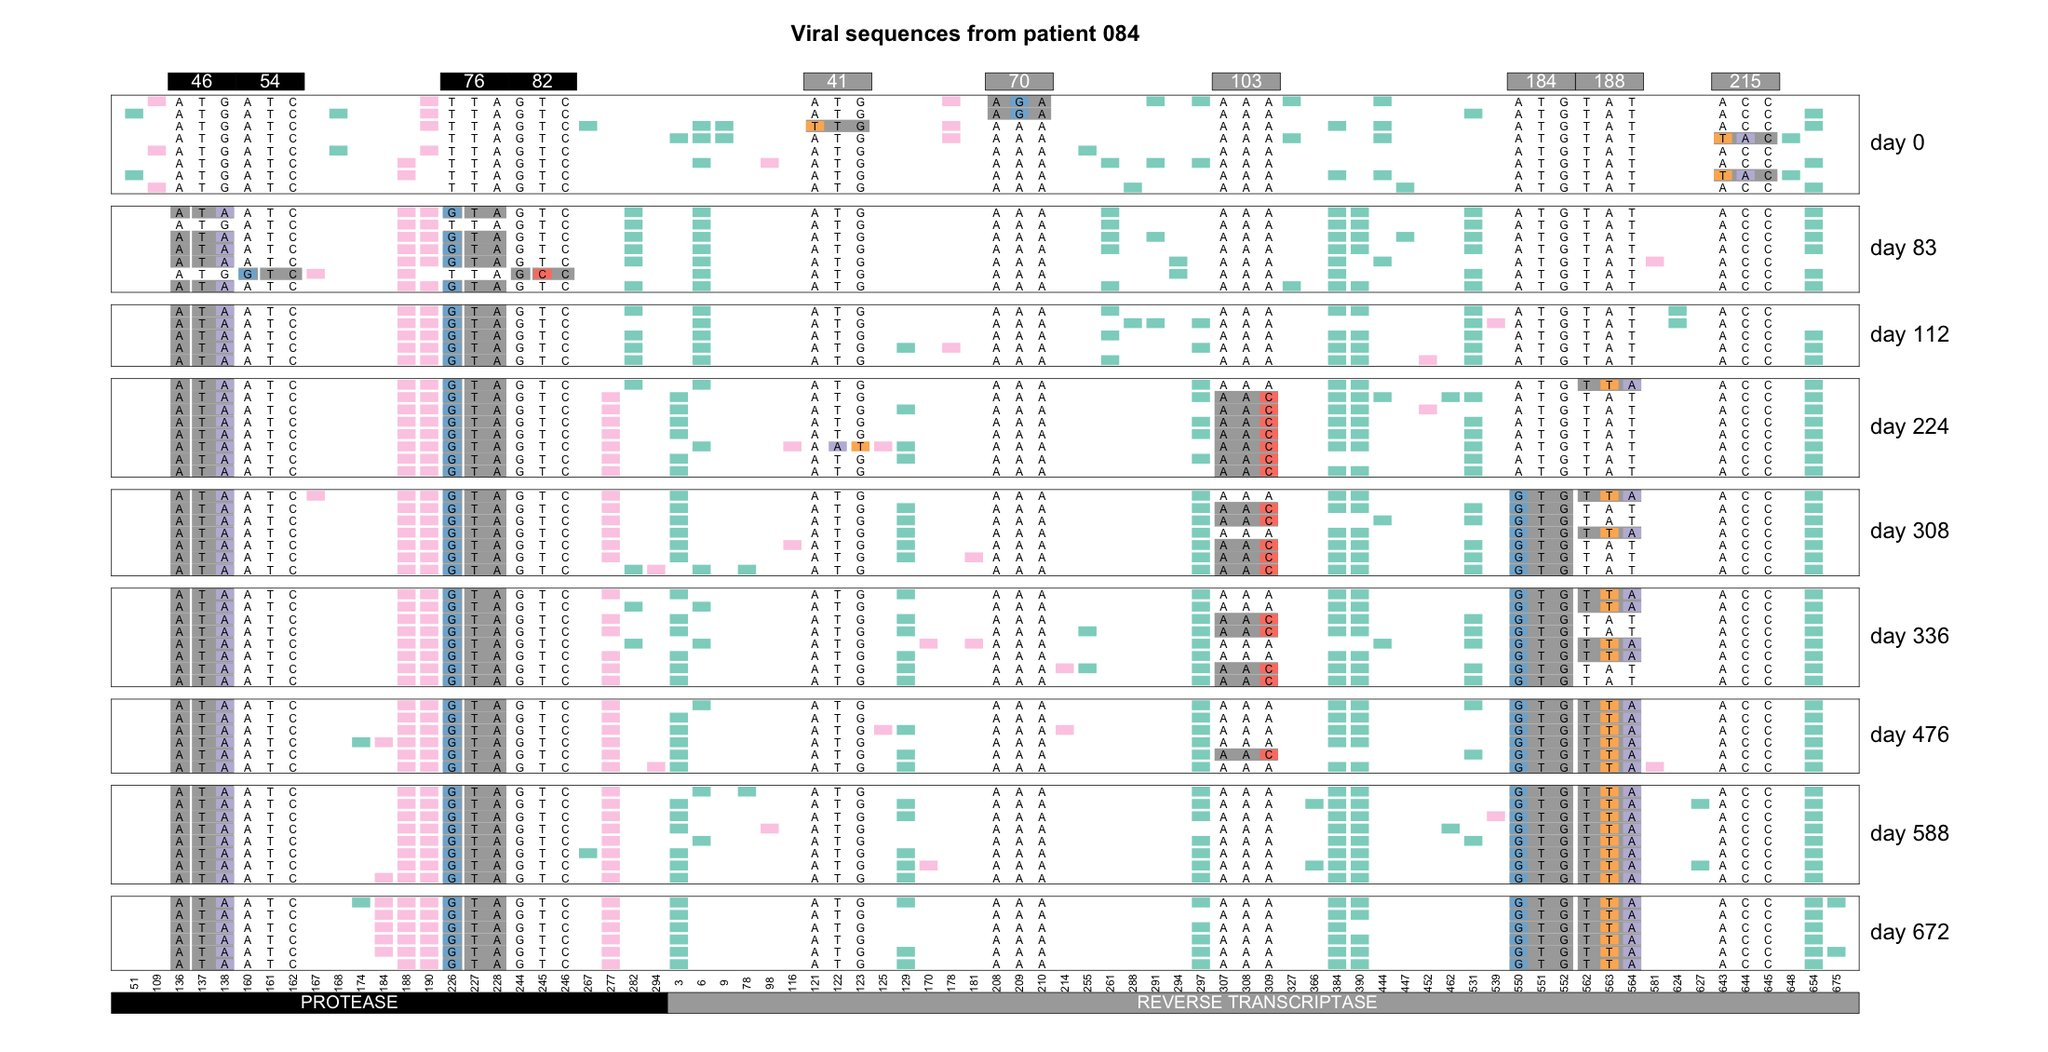
\includegraphics[width =  \textwidth]{Journal_figs/recom_selection/Pleuni_HIV_interference/DdwdkVeVMAA7t-V.jpg}
\end{center}
\caption{} \label{fig:HIV_interference}  %é
\end{figure}

\begin{figure}
\begin{center}
  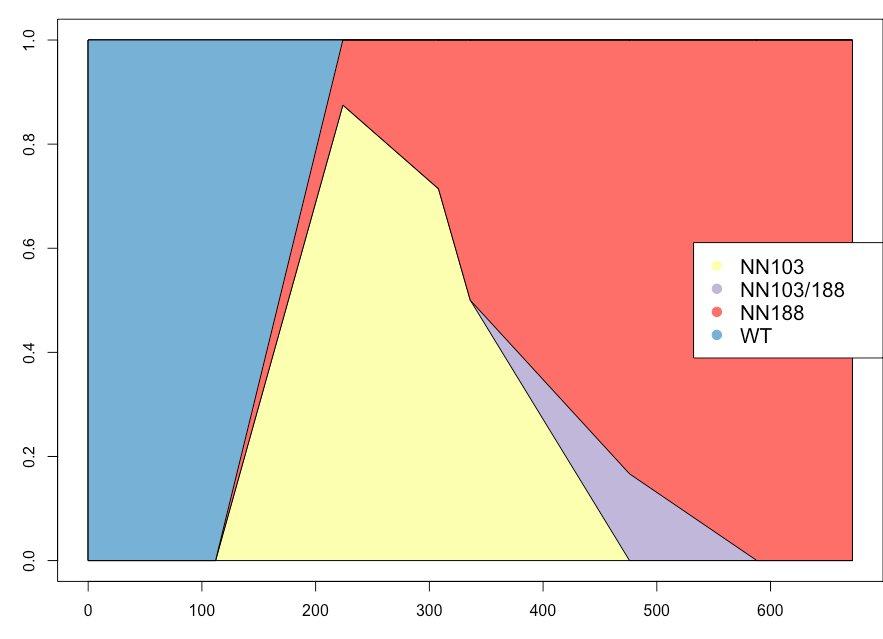
\includegraphics[width = 0.8 \textwidth]{Journal_figs/recom_selection/Pleuni_HIV_interference/DdweQyxU0AA7mXe.jpg}
\end{center}
\caption{} \label{fig:HIV_interference_M}  %é
\end{figure}


%In this simple model of viability selection
